\section{Dataset}
The DIV2K dataset with DIVerse 2K resolution high quality images collected from Internet. It has 1000 images with considerable higher resolution than the popular datasets. The images were obtained by paying special attention to the image quality,
to the diversity of sources (sites and cameras), to the image
contents and to the copyrights. All the 1000 images are 2K resolution, that is they have 2K pixels on at least one of the axes(vertical or horizontal). Since the most common
magnification factors are of $×2$, $×3$ and $×4$ the images are cropped to multiples of 12 pixels on both axes. The images are of high quality both aesthetically and in the terms of small amounts of noise and other corruptions (like blur and color shifts). The images are collected from dozens of sites. A preference was made for sites with freely shared high
quality photography. DIV2K covers a large diversity of contents,ranging from people, handmade objects and environments(cities, villages), to flora and fauna, and natural sceneries including underwater and dim light conditions. After collecting the images they randomly generated partitions of 800 train, 100 validation and 100 test images until they achieved a good balance firstly in visual contents and then on the state of the art measurements like entropy,PSNR etc.
\begin{figure}[h]
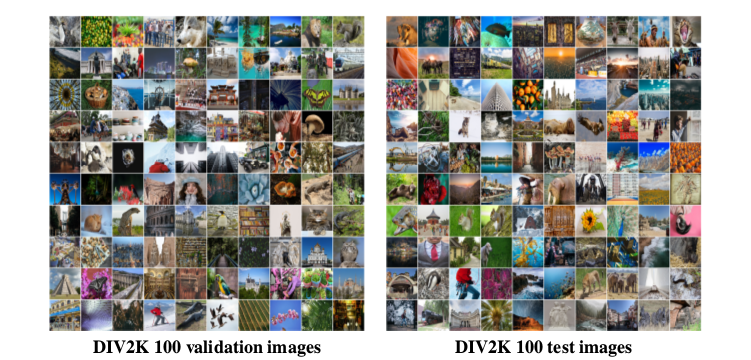
\includegraphics[scale=0.5]{dataset}
\caption{Visualization of proposed DIV2K validation and test images. DIV2K contains also 800 train images.}
\end{figure}